\section{The Incidence Matrices and Hodge Matrices}

The incidence matrices $\mathbb{E}$ and the Hodge matrices $\mathbb{H}$ are derived using the mesh introduced in the Section \ref{sec:discretization}. The incidence and Hodge matrices derived in this section are exclusively valid for the mesh shown in Figure \ref{fig:outerGrid} and Figure \ref{fig:innerGrid}. That is, the validity is limited to the rather coarse spacing of $n = 3$. However, the format of those matrices belonging to denser grids can be correctly deduced by careful analysis of the matrix structure at $n = 3$, which is of course what we are after.

\subsection{$\tilde{\mathbb{E}}^{(2,1)}$}

The application of the incidence matrix $\tilde{\mathbb{E}}^{(2,1)}$ to the 1-cochain that represent flux, $\mathbf{\tilde{u}}^{(1)}$, yields the rate of mass production in the plane enclosed by those line segments, $\mathbf{\tilde{S}}^{(2)}$. Let us construct a linear equation for each of the planes $\tilde{s}_{i,j}$ in the mesh:
\begin{equation}
    \begin{split}
        \tilde{s}_{0,0} &= -\tilde{u}_{0,0} + \tilde{u}_{1,0} - \tilde{v}_{0,0} + \tilde{v}_{0,1} \\
        \tilde{s}_{1,0} &= -\tilde{u}_{1,0} + \tilde{u}_{2,0} - \tilde{v}_{1,0} + \tilde{v}_{1,1} \\
        &\vdots \\
        \tilde{s}_{2,2} &= -\tilde{u}_{2,2} + \tilde{u}_{3,2} - \tilde{v}_{2,2} + \tilde{v}_{2,3} \\
    \end{split}
    \label{eq:tsijEquations}
\end{equation}
Equation \eqref{eq:tsijEquations} expressed in matrix notation becomes
\begin{equation}
    \mathbf{\tilde{s}}^{(2)} = \tilde{\mathbb{E}}^{(2,1)} \mathbf{\tilde{u}}^{(1)}
    \label{eq:tE21}
\end{equation}
The mass flow rates $\tilde{u}_{i,j}$ and $\tilde{v}_{i,j}$ adjacent to the boundary of the unit square are known because the boundary conditions of the problem are known. The matrices in the right-hand side of Equation \eqref{eq:tE21} can be split into a matrix of unknowns and into a matrix of knows. Splitting the matrix into two parts yields
\begin{equation}
    \mathbf{\tilde{s}}^{(2)} = \tilde{\mathbb{E}}^{(2,1)} \mathbf{\tilde{u}}^{(1)} + \tilde{\mathbb{E}}^{(2,1)}_{\text{known}} \mathbf{\tilde{u}}^{(1)}_{\text{known}}
\end{equation}
where
\begin{equation}
    \setlength{\arraycolsep}{0pt}
    \tilde{\mathbb{E}}^{(2,1)} =
    \left[
    \begin{array}{cccccccccccc}
        \w{1} & \d & \d & \d & \d & \d & \w{1} & \d & \d & \d & \d & \d \\
        -1 & \w{1} & \d & \d & \d & \d & \d & \w{1} & \d & \d & \d & \d \\
        \d & -1 & \d & \d & \d & \d & \d & \d & \w{1} & \d & \d & \d \\
        \d & \d & \w{1} & \d & \d & \d & -1 & \d & \d & \w{1} & \d & \d \\
        \d & \d & -1 & \w{1} & \d & \d & \d & -1 & \d & \d & \w{1} & \d \\
        \d & \d & \d & -1 & \d & \d & \d & \d & -1 & \d & \d & \w{1} \\
        \d & \d & \d & \d & \w{1} & \d & \d & \d & \d & -1 & \d & \d \\
        \d & \d & \d & \d & -1 & \w{1} & \d & \d & \d & \d & -1 & \d \\
        \d & \d & \d & \d & \d & -1 & \d & \d & \d & \d & \d & -1 \\
    \end{array}
    \right]
\end{equation}

\begin{flalign}
    & \text{and} &
    \setlength{\arraycolsep}{0pt}
    \tilde{\mathbb{E}}^{(2,1)}_{\text{known}} =
    \left[
    \begin{array}{cccccccccccc}
        -1 & \d & \d & \d & \d & \d & -1 & \d & \d & \d & \d & \d \\
        \d & \d & \d & \d & \d & \d & \d & -1 & \d & \d & \d & \d \\
        \d & \w{1} & \d & \d & \d & \d & \d & \d & -1 & \d & \d & \d \\
        \d & \d & -1 & \d & \d & \d & \d & \d & \d & \d & \d & \d \\
        \d & \d & \d & \d & \d & \d & \d & \d & \d & \d & \d & \d \\
        \d & \d & \d & \w{1} & \d & \d & \d & \d & \d & \d & \d & \d \\
        \d & \d & \d & \d & -1 & \d & \d & \d & \d & \w{1} & \d & \d \\
        \d & \d & \d & \d & \d & \d & \d & \d & \d & \d & \w{1} & \d \\
        \d & \d & \d & \d & \d & \w{1} & \d & \d & \d & \d & \d & \w{1} \\
    \end{array}
    \right] &&
\end{flalign}
(\textit{Note:} The zero elements are replaced by dots to make the non-zero elements stand out. This turns out to be useful because it makes it far easier to see the structure of the matrices in the blink of an eye.)

Notice that every column of $\tilde{\mathbb{E}}^{(2,1)}$ contains two non-zero elements. The number of non-zero elements (NNZ) in $\tilde{\mathbb{E}}^{(2,1)}$ therefore equals
\begin{equation}
    \mbox{NNZ}(\tilde{\mathbb{E}}^{(2,1)}) = 2 \cdot 4 n = 8 n
\end{equation}
Also notice that every column of $\tilde{\mathbb{E}}^{(2,1)}_{\text{known}}$ contains one non-zero element. Thus,
\begin{equation}
    \mbox{NNZ}(\tilde{\mathbb{E}}^{(2,1)}_{\text{known}}) = 4 n
\end{equation}
It should be no surprise here that the extreme sparsity of these indicence matrices is a property worth exploiting.

\subsection{$\mathbb{E}^{(1,0)}$}

The incidence matrix $\mathbb{E}^{(1,0)}$ maps an inner-oriented 0-cochain to an inner-oriented 1-cochain. Let us create a linear equation for each of the line segments $u_{(i,j)}$ in the inner-oriented grid, considering that the points $P_{(i,j)}$ are sink-like. The equations are given by
\begin{equation}
    \begin{split}
        u_{1,1} &= -p_{1,1} + p_{2,1} \\
        u_{2,1} &= -p_{2,1} + p_{3,1} \\
        &\vdots \\
        u_{2,3} &= -p_{2,3} + p_{3,3} \\
        v_{1,1} &= -p_{1,1} + p_{1,2} \\
        v_{2,1} &= -p_{2,1} + p_{2,2} \\
        &\vdots \\
        v_{3,2} &= -p_{3,2} + p_{3,3}
    \end{split}
    \label{eq:E10list}
\end{equation}
Equation \eqref{eq:E10list} can be written in matrix notation as
\begin{equation}
    \mathbf{u}^{(1)} = \mathbb{E}^{(1,0)} \mathbf{p}^{(0)}
\end{equation}
where
\begin{equation}
    \setlength{\arraycolsep}{0pt}
    \mathbb{E}^{(1,0)} =
    \left[
    \begin{array}{ccccccccc}
        -1 & \w{1} & \d & \d & \d & \d & \d & \d & \d \\
        \d & -1 & \w{1} & \d & \d & \d & \d & \d & \d \\
        \d & \d & \d & -1 & \w{1} & \d & \d & \d & \d \\
        \d & \d & \d & \d & -1 & \w{1} & \d & \d & \d \\
        \d & \d & \d & \d & \d & \d & -1 & \w{1} & \d \\
        \d & \d & \d & \d & \d & \d & \d & -1 & \w{1} \\
        -1 & \d & \d & \w{1} & \d & \d & \d & \d & \d \\
        \d & -1 & \d & \d & \w{1} & \d & \d & \d & \d \\
        \d & \d & -1 & \d & \d & \w{1} & \d & \d & \d \\
        \d & \d & \d & -1 & \d & \d & \w{1} & \d & \d \\
        \d & \d & \d & \d & -1 & \d & \d & \w{1} & \d \\
        \d & \d & \d & \d & \d & -1 & \d & \d & \w{1}
    \end{array}
    \right]
\end{equation}

It is important to recognize that
\begin{equation}
    \mathbb{E}^{(1,0)} = -\left(\tilde{\mathbb{E}}^{(2,1)}\right)^T
\end{equation}
because this little shortcut will save us some computational effort.

\subsection{$\mathbb{E}^{(2,1)}$}

The incidence matrix $\mathbb{E}^{(2,1)}$ maps an inner-oriented 1-cochain to an inner-oriented 2-cochain. That is, it maps circulation along line segments to vorticity in the planes enclosed by those line segments. The derivation of $\mathbb{E}^{(2,1)}$ is straightforward: add the circulation along those line segments that share a common orientation with the plane and subtract the circulation along those line segments whose orientation opposes the orientation of the plane. Executing this procedure for all planes $\xi_{i,j}$, we have
\begin{equation}
    \begin{split}
        \mathbf{\xi}_{0,0} &= u_{0,0} - u_{0,1} - v_{0,0} + v_{1,0} \\
        \mathbf{\xi}_{1,0} &= u_{1,0} - u_{1,1} - v_{1,0} + v_{2,0} \\
        &\vdots \\
        \mathbf{\xi}_{3,3} &= u_{3,3} - u_{3,4} - v_{3,3} + v_{4,3}
    \end{split}
    \label{eq:xiijEquations}
\end{equation}
which is in accordance to the formula
\begin{equation}
    \xi_{i,j} = u_{i,j} - u_{i,j+1} - v_{i,j} + v_{i+1,j}
\end{equation}
Equation \eqref{eq:xiijEquations} written in matrix notation yields
\begin{equation}
    \mathbf{\xi}^{(2)} = \mathbb{E}^{(2,1)} \mathbf{u}^{(1)}
\end{equation}

The velocities adjacent to the boundary are again known because the boundary conditions of the problem are known. Splitting the incidence matrix $\mathbb{E}^{(2,1)}$ into a matrix of unknowns and into a matrix of knows yields
\begin{equation}
    \mathbf{\xi}^{(2)} = \mathbb{E}^{(2,1)} \mathbf{u}^{(1)} + \mathbb{E}^{(2,1)}_{\text{known}} \mathbf{u}^{(1)}_{\text{known}}
    \label{eq:xi}
\end{equation}
where
\begin{equation}
    \setlength{\arraycolsep}{0pt}
    \mathbb{E}^{(2,1)} =
    \left[
    \begin{array}{cccccccccccc}
        \d & \d & \d & \d & \d & \d & \d & \d & \d & \d & \d & \d \\
        -1 & \d & \d & \d & \d & \d & \d & \d & \d & \d & \d & \d \\
        \d & -1 & \d & \d & \d & \d & \d & \d & \d & \d & \d & \d \\
        \d & \d & \d & \d & \d & \d & \d & \d & \d & \d & \d & \d \\
        \d & \d & \d & \d & \d & \d & \w{1} & \d & \d & \d & \d & \d \\
        \w{1} & \d & -1 & \d & \d & \d & -1 & \w{1} & \d & \d & \d & \d \\
        \d & \w{1} & \d & -1 & \d & \d & \d & -1 & \w{1} & \d & \d & \d \\
        \d & \d & \d & \d & \d & \d & \d & \d & -1 & \d & \d & \d \\
        \d & \d & \d & \d & \d & \d & \d & \d & \d & \w{1} & \d & \d \\
        \d & \d & \w{1} & \d & -1 & \d & \d & \d & \d & -1 & \w{1} & \d \\
        \d & \d & \d & \w{1} & \d & -1 & \d & \d & \d & \d & -1 & \w{1} \\
        \d & \d & \d & \d & \d & \d & \d & \d & \d & \d & \d & -1 \\
        \d & \d & \d & \d & \d & \d & \d & \d & \d & \d & \d & \d \\
        \d & \d & \d & \d & \w{1} & \d & \d & \d & \d & \d & \d & \d \\
        \d & \d & \d & \d & \d & \w{1} & \d & \d & \d & \d & \d & \d \\
        \d & \d & \d & \d & \d & \d & \d & \d & \d & \d & \d & \d
    \end{array}
    \right]
\end{equation}
and
\begin{multline}
    \mathbb{E}^{(2,1)}_{\text{known}} = \\
    \setlength{\arraycolsep}{0pt}
    \left[
    \begin{array}{cccccccccccccccccccccccccccc}
        \w{1} & \d & \d & \d & -1 & \d & \d & \d & \d & \d & \d & \d & \d & \d &
        -1 & \w{1} & \d & \d & \d & \d & \d & \d & \d & \d & \d & \d & \d & \d \\
        \d & \w{1} & \d & \d & \d & \d & \d & \d & \d & \d & \d & \d & \d & \d &
        \d & -1 & \w{1} & \d & \d & \d & \d & \d & \d & \d & \d & \d & \d & \d \\
        \d & \d & \w{1} & \d & \d & \d & \d & \d & \d & \d & \d & \d & \d & \d &
        \d & \d & -1 & \w{1} & \d & \d & \d & \d & \d & \d & \d & \d & \d & \d \\
        \d & \d & \d & \w{1} & \d & -1 & \d & \d & \d & \d & \d & \d & \d & \d &
        \d & \d & \d & -1 & \w{1} & \d & \d & \d & \d & \d & \d & \d & \d & \d \\
        \d & \d & \d & \d & \w{1} & \d & -1 & \d & \d & \d & \d & \d & \d & \d &
        \d & \d & \d & \d & \d & -1 & \d & \d & \d & \d & \d & \d & \d & \d \\
        \d & \d & \d & \d & \d & \d & \d & \d & \d & \d & \d & \d & \d & \d &
        \d & \d & \d & \d & \d & \d & \d & \d & \d & \d & \d & \d & \d & \d \\
        \d & \d & \d & \d & \d & \d & \d & \d & \d & \d & \d & \d & \d & \d &
        \d & \d & \d & \d & \d & \d & \d & \d & \d & \d & \d & \d & \d & \d \\
        \d & \d & \d & \d & \d & \w{1} & \d & -1 & \d & \d & \d & \d & \d & \d &
        \d & \d & \d & \d & \d & \d & \w{1} & \d & \d & \d & \d & \d & \d & \d \\
        \d & \d & \d & \d & \d & \d & \w{1} & \d & -1 & \d & \d & \d & \d & \d &
        \d & \d & \d & \d & \d & \d & \d & -1 & \d & \d & \d & \d & \d & \d \\
        \d & \d & \d & \d & \d & \d & \d & \d & \d & \d & \d & \d & \d & \d &
        \d & \d & \d & \d & \d & \d & \d & \d & \d & \d & \d & \d & \d & \d \\
        \d & \d & \d & \d & \d & \d & \d & \d & \d & \d & \d & \d & \d & \d &
        \d & \d & \d & \d & \d & \d & \d & \d & \d & \d & \d & \d & \d & \d \\
        \d & \d & \d & \d & \d & \d & \d & \w{1} & \d & -1 & \d & \d & \d & \d &
        \d & \d & \d & \d & \d & \d & \d & \d & \w{1} & \d & \d & \d & \d & \d \\
        \d & \d & \d & \d & \d & \d & \d & \d & \w{1} & \d & -1 & \d & \d & \d &
        \d & \d & \d & \d & \d & \d & \d & \d & \d & -1 & \w{1} & \d & \d & \d \\
        \d & \d & \d & \d & \d & \d & \d & \d & \d & \d & \d & -1 & \d & \d &
        \d & \d & \d & \d & \d & \d & \d & \d & \d & \d & -1 & \w{1} & \d & \d \\
        \d & \d & \d & \d & \d & \d & \d & \d & \d & \d & \d & \d & -1 & \d &
        \d & \d & \d & \d & \d & \d & \d & \d & \d & \d & \d & -1 & \w{1} & \d \\
        \d & \d & \d & \d & \d & \d & \d & \d & \d & \w{1} & \d & \d & \d & -1 &
        \d & \d & \d & \d & \d & \d & \d & \d & \d & \d & \d & \d & -1 & \w{1} \\
    \end{array}
    \right]
\end{multline}

The product $\mathbb{E}^{(2,1)}_{\text{known}} \mathbf{u}^{(1)}_{\text{known}}$ can be evaluated because both factors are known. Equation \eqref{eq:xi} reduces to
\begin{equation}
    \mathbf{\xi}^{(2)} = \mathbb{E}^{(2,1)} \mathbf{u}^{(1)} + \mathbf{u}^{(1)}_{\text{prescribed}}
\end{equation}
Note that each column of the matrix $\mathbb{E}^{(2,1)}$ contains two non-zero elements. Therefore, the total number of non-zero elements in $\mathbb{E}^{(2,1)}$ amounts to
\begin{equation}
    \mbox{NNZ}(\mathbb{E}^{(2,1)}) = 2 \cdot 4 \cdot n = 8n
\end{equation}


\subsection{$\tilde{\mathbb{E}}^{(1,0)}$}

The incidence matrix $\tilde{\mathbb{E}}^{(1,0)}$ maps an outer-oriented 0-cochain to an outer-oriented 1-cochain. That is, it maps values of the stream function located at the discrete points of the mesh to flux through the line segments. Deriving $\tilde{\mathbb{E}}^{(1,0)}$ is again straightforward; each of the line segments is bounded by two points. The flux through a line is equal to the sum of the values of the stream function at the bounding points. Add values at points whose orientation is equal to that of the line and subtract values at points whose orientation opposes the orientation of the line. Repeating this process for each of the line segments, we have
\begin{equation}
    \begin{split}
        \tilde{u}_{1,0} &= -\tilde{\psi}_{1,0} + \tilde{\psi}_{1,1} \\
        \tilde{u}_{2,0} &= -\tilde{\psi}_{3,0} + \tilde{\psi}_{2,1} \\
        &\vdots \\
        \tilde{u}_{2,2} &= -\tilde{\psi}_{2,2} + \tilde{\psi}_{2,3} \\
        \tilde{v}_{0,1} &= \tilde{\psi}_{0,1} - \tilde{\psi}_{1,1} \\
        \tilde{v}_{1,1} &= \tilde{\psi}_{1,1} - \tilde{\psi}_{2,1} \\
        &\vdots \\
        \tilde{v}_{2,2} &= \tilde{\psi}_{2,2} - \tilde{\psi}_{3,2}
    \end{split}
    \label{eq:tuij}
\end{equation}
Expressing Equation \eqref{eq:tuij} in matrix notation yields
\begin{equation}
    \mathbf{\tilde{u}} = \mathbb{\tilde{E}}^{(1,0)} \mathbf{\tilde{\psi}}
\end{equation}
where
\begin{equation}
    \setlength{\arraycolsep}{0pt}
    \mathbb{\tilde{E}}^{(1,0)} =
    \left[
    \begin{array}{cccccccccccccccc}
        \w{\d} & -1 & \d & \w{\d} & \d & \w{1} & \d & \d & \d & \d & \d & \w{\d} & \w{\d} & \d & \d & \w{\d} \\
        \d & \d & -1 & \d & \d & \d & \w{1} & \d & \d & \d & \d & \d & \d & \d & \d & \d \\
        \d & \d & \d & \d & \d & -1 & \d & \d & \d & \w{1} & \d & \d & \d & \d & \d & \d \\
        \d & \d & \d & \d & \d & \d & -1 & \d & \d & \d & \w{1} & \d & \d & \d & \d & \d \\
        \d & \d & \d & \d & \d & \d & \d & \d & \d & -1 & \d & \d & \d & \w{1} & \d & \d \\
        \d & \d & \d & \d & \d & \d & \d & \d & \d & \d & -1 & \d & \d & \d & \w{1} & \d \\
        \d & \d & \d & \d & \w{1} & -1 & \d & \d & \d & \d & \d & \d & \d & \d & \d & \d \\
        \d & \d & \d & \d & \d & \w{1} & -1 & \d & \d & \d & \d & \d & \d & \d & \d & \d \\
        \d & \d & \d & \d & \d & \d & \w{1} & -1 & \d & \d & \d & \d & \d & \d & \d & \d \\
        \d & \d & \d & \d & \d & \d & \d & \d & \w{1} & -1 & \d & \d & \d & \d & \d & \d \\
        \d & \d & \d & \d & \d & \d & \d & \d & \d & \w{1} & -1 & \d & \d & \d & \d & \d \\
        \d & \d & \d & \d & \d & \d & \d & \d & \d & \d & \w{1} & -1 & \d & \d & \d & \d
    \end{array}
    \right]
\end{equation}
Also take note that
\begin{equation}
    \mathbb{\tilde{E}}^{(1,0)} = \left(\mathbb{E}^{(2,1)}\right)^T
\end{equation}
which will again save us some computational effort.

\subsection{$\mathbb{H}^{(\tilde{1},1)}$ and $\mathbb{H}^{(1,\tilde{1})}$}

The Hodge matrix $\mathbb{H}^{(\tilde{1},1)}$ represents a linear map between between the flux through a line segment and the circulation along a line segment. Its inverse, $\mathbb{H}^{(1,\tilde{1})}$, represents a linear map between the circulation along a line segment and the flux through a line segment. The cirulation along a line segment is equal to the velocity along that line segment times the lenght of the line segment. Or, expressed as a function of flux:
\begin{equation}
    \text{ciculation along $L_a$} = \underbrace{\frac{\text{mass flow through $L_b$}}{\text{length of $L_b$}}}_{\text{velocity}} \cdot \underbrace{\vphantom{\frac{\text{mass flow through $L_b$}}{\text{length of $L_b$}}}\text{length of $L_a$}}_{\text{length}}
\end{equation}
Let us look at a specific example. The circulation along the line segment $u_{1,1}$ in Figure \ref{fig:innerGrid} is given by
\begin{equation}
    u_{2,1} = \frac{\tilde{u}_{2,0}}{\tilde{h}_0} h_2 = \frac{h_2}{\tilde{h}_0} \tilde{u}_{2,0}
    \label{eq:H1t1Example}
\end{equation}
In general, the circulation along the line segments $u_{i,j}$ and $v_{i,j}$ can be found in accordance to the formulas
\begin{flalign}
    \stepcounter{equation}
    \tag{{\theequation}a}
    & & u_{i,j} = \frac{h_i}{\tilde{h}_{j-1}} \tilde{u}_{i,j-1} && \label{eq:H1t1FormulaU} \\
    \tag{{\theequation}b}
    &\text{and}& v_{i,j} = \frac{h_j}{\tilde{h}_{i-1}} \tilde{v}_{i-1,j} \label{eq:H1t1FormulaV} &&
\end{flalign}
Equations \eqref{eq:H1t1FormulaU} and \eqref{eq:H1t1FormulaV} expressed in matrix notation yield
\begin{equation}
    \mathbf{u}^{(1)} = \mathbb{H}^{(1,\tilde{1})} \mathbf{\tilde{u}}^{(1)}
\end{equation}
The matrix $\mathbb{H}^{(1,\tilde{1})}$ is a diagonal matrix since it represents a linear operation.

\subsection{$\mathbb{H}^{(\tilde{0},2)}$ and $\mathbb{H}^{(2,\tilde{0})}$}

The Hodge matrix $\mathbb{H}^{(\tilde{0},2)}$ maps the vorticity associated with an inner-oriented 2-cochain to the stream function associated with an outer-oriented 0-cochain. This amounts to simply deviding the inner-oriented 2-cochain by its area:
\begin{equation}
    \tilde{\psi}_{i,j} = \left( h_i h_j \right)^{-1} \xi_{i,j}
    \label{eq:psiij}
\end{equation}
Equation \eqref{eq:psiij} written in matrix notation yields
\begin{equation}
    \mathbf{\tilde{\psi}}^{(0)} = \mathbb{H}^{(\tilde{0},2)} \mathbf{\xi}^{(2)}
\end{equation}
where $\mathbb{H}^{(\tilde{0},2)}$ is again a diagonal matrix. Its inverse, $\mathbb{H}^{(2,\tilde{0})}$, represents a linear map between an outer-oriented 0-cochain and an inner-oriented 2-cochain.

\subsection{The Convective Term}

The derivation of the convective term, $\mathbf{u}^{(1)} \times \mathbf{\xi}^{(2)}$, is not quite straightforward. The convective term is an exterior product of a 1-cochain and a 2-cochain. If $\mathbf{\xi}^{(2)}$ and $\mathbf{u}^{(1)}$ are given by
\begin{flalign}
    & & \mathclap{\mathbf{\xi}^{(2)} = \xi \; dx \; dy} && \\
    & \text{and} & \mathclap{\mathbf{u}^{(1)} = u \frac{\partial}{\partial x} + v \frac{\partial}{\partial y}} &&
\end{flalign}
respectively, then the exterior product yields
\begin{equation}
    \mathbf{u}^{(1)} \times \mathbf{\xi}^{(2)} = u \xi \; dy - v \xi \; dx
\end{equation}

As an example, let us compute the convection through the line segment $u_{1,1}$. Line segment $u_{1,1}$ is shown in Figure \ref{fig:convectionExample} along with the adjacent lines and planes that are involved in the computation.
\begin{figure}[ht]
    \centering
    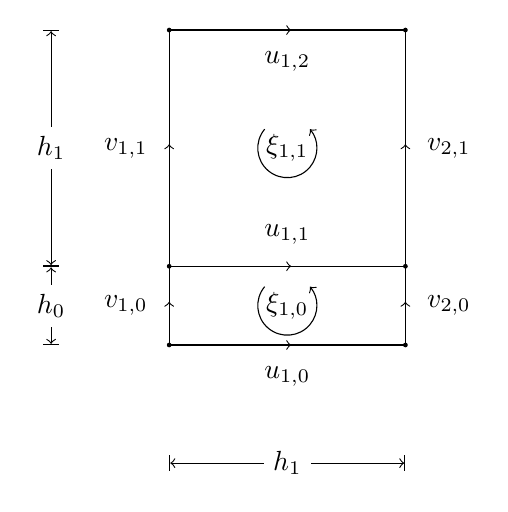
\begin{tikzpicture}
        % Draw scale
        \foreach \ia/\ib/\count in {0/1/0, 1/4/1} {
            \draw [|<->|] (-0.5,\ia) -- (-0.5,\ib) node [midway,fill=white] {$h_\count$};
        }
        \foreach \ia/\ib/\count in {1/4/1} {
            \draw [|<->|] (\ia,-1.5) -- (\ib,-1.5) node [midway,fill=white] {$h_\count$};
        }
        % Draw lines
        \draw (1,0) -- (1,4);
        \draw (4,0) -- (4,4);
        \draw (1,1) -- (4,1);
        \draw (1,1) -- (4,1);
        \draw (1,0) -- (4,0);
        \draw (1,4) -- (4,4);
        % Six corner points
        \fill (1,0) circle (0.03);
        \fill (4,0) circle (0.03);
        \fill (1,4) circle (0.03);
        \fill (4,4) circle (0.03);
        \fill (1,1) circle (0.03);
        \fill (4,1) circle (0.03);
        % Draw v
        \foreach \x/\i in {1/1} {
            \foreach \y/\j in {0.5/0, 2.5/1} {
                \draw [->] (\x,\y) -- (\x,\y+0.05);
                \node[left=1ex] at (\x,\y) {$v_{\i,\j}$};
            }
        }
        \foreach \x/\i in {4/2} {
            \foreach \y/\j in {0.5/0, 2.5/1} {
                \draw [->] (\x,\y) -- (\x,\y+0.05);
                \node[right=1ex] at (\x,\y) {$v_{\i,\j}$};
            }
        }
        % Draw u
        \foreach \x/\i in {0/0, 4/2} {
            \foreach \y/\j in {2.5/1} {
                \draw [->] (\y,\x) -- (\y+0.05,\x);
                \node[below=1ex] at (\y,\x) {$u_{\j,\i}$};
            }
        }
        \foreach \x/\i in {1/1} {
            \foreach \y/\j in {2.5/1} {
                \draw [->] (\y,\x) -- (\y+0.05,\x);
                \node[above=1ex] at (\y,\x) {$u_{\j,\i}$};
            }
        }
        % Draw xi
        \foreach \x/\i in {2.5/1} {
            \foreach \y/\j in {0.5/0, 2.5/1} {
                \draw [->] (\x,\y) ++(140:0.375) arc (-220:40:0.375);
                \node at (\x,\y) {$\xi_{\i,\j}$};
            }
        }
    \end{tikzpicture}
    \caption{Convection through $u_{1,1}$.}
    \label{fig:convectionExample}
\end{figure}

Because $u_{1,1}$ is a strictly horizontal line segment, we do not need to consider the horizontal component of the convection through this line segment. Computing the mean vertical velocity in the plane below the line $u_{1,1}$ and multiplying it by $\tilde{\psi}_{1,0}$, we have
\begin{equation}
    -\frac{1}{2} \left( \frac{v_{1,0}}{h_0} + \frac{v_{2,0}}{h_0} \right) \tilde{\psi}_{1,0}
    \label{eq:planeBelow}
\end{equation}
For the plane above the line $u_{1,1}$, we have
\begin{equation}
    -\frac{1}{2} \left( \frac{v_{1,1}}{h_1} + \frac{v_{2,1}}{h_1} \right) \tilde{\psi}_{1,1}
    \label{eq:planeAbove}
\end{equation}
The average of Equations \eqref{eq:planeBelow} and \eqref{eq:planeAbove} multiplied by the length of $u_{1,1}$ yields the convection accross $u_{1,1}$:
\begin{flalign}
    & & \mathclap{\frac{1}{2} \left[ -\frac{1}{2} \left( \frac{v_{1,0}}{h_0} + \frac{v_{2,0}}{h_0} \right) \tilde{\psi}_{1,0} - \frac{1}{2} \left( \frac{v_{1,1}}{h_1} + \frac{v_{2,1}}{h_1} \right) \tilde{\psi}_{1,1} \right] h_1} && \\
    & \text{or} & \mathclap{-\frac{h_1}{4 h_0} \left( v_{1,0} + v_{2,0} \right) \tilde{\psi}_{1,0} - \frac{h_1}{4 h_1} \left( v_{1,1} + v_{2,1} \right) \tilde{\psi}_{1,1}} &&
\end{flalign}
The final multipliplication by $h_1$, the length of the line segment $u_{1,1}$, is neseccary because the momentum equation is a 1-form equation. That is, all terms of the momentum equation must ultimately be expressed as inner-oriented 1-cochains. Repetition of the above procedure for all line segments $u_{i,j}$ and $v_{i,j}$ yields
\begin{equation}
    \mbox{convection}
    =
    \begin{bmatrix}
    - \frac{\tilde{h}_1}{4 \tilde{h}_0} \left( v_{1,0} + v_{2,0} \right) \psi_{1,0} - \frac{\tilde{h}_1}{4 \tilde{h}_1} \left( v_{1,1} + v_{2,1} \right) \psi_{1,1} \\

    - \frac{\tilde{h}_2}{4 \tilde{h}_0} \left( v_{2,0} + v_{3,0} \right) \psi_{2,0} - \frac{\tilde{h}_2}{4 \tilde{h}_1} \left( v_{2,1} + v_{3,1} \right) \psi_{2,1} \\

    - \frac{\tilde{h}_1}{4 \tilde{h}_1} \left( v_{1,1} + v_{2,1} \right) \psi_{1,1} - \frac{\tilde{h}_1}{4 \tilde{h}_2} \left( v_{1,2} + v_{2,2} \right) \psi_{1,2} \\

    - \frac{\tilde{h}_2}{4 \tilde{h}_1} \left( v_{2,1} + v_{3,1} \right) \psi_{2,1} - \frac{\tilde{h}_2}{4 \tilde{h}_2} \left( v_{2,2} + v_{3,2} \right) \psi_{2,2} \\

    - \frac{\tilde{h}_1}{4 \tilde{h}_2} \left( v_{1,2} + v_{2,2} \right) \psi_{1,2} - \frac{\tilde{h}_1}{4 \tilde{h}_3} \left( v_{1,3} + v_{2,3} \right) \psi_{1,3} \\

    - \frac{\tilde{h}_2}{4 \tilde{h}_2} \left( v_{2,2} + v_{3,2} \right) \psi_{2,2} - \frac{\tilde{h}_2}{4 \tilde{h}_3} \left( v_{2,3} + v_{3,3} \right) \psi_{2,3} \\

    \frac{\tilde{h}_0}{4 \tilde{h}_0} \left( u_{0,1} + u_{0,2} \right) \psi_{0,1} + \frac{\tilde{h}_0}{4 \tilde{h}_1} \left( u_{1,1} + u_{1,2} \right) \psi_{1,1} \\

    \frac{\tilde{h}_1}{4 \tilde{h}_1} \left( u_{1,1} + u_{1,2} \right) \psi_{1,1} + \frac{\tilde{h}_1}{4 \tilde{h}_2} \left( u_{2,1} + u_{2,2} \right) \psi_{2,1} \\

    \frac{\tilde{h}_2}{4 \tilde{h}_2} \left( u_{2,1} + u_{2,2} \right) \psi_{2,1} + \frac{\tilde{h}_2}{4 \tilde{h}_3} \left( u_{3,1} + u_{3,2} \right) \psi_{3,1} \\

    \frac{\tilde{h}_0}{4 \tilde{h}_0} \left( u_{0,2} + u_{0,3} \right) \psi_{0,2} + \frac{\tilde{h}_0}{4 \tilde{h}_1} \left( u_{1,2} + u_{1,3} \right) \psi_{1,2} \\

    \frac{\tilde{h}_1}{4 \tilde{h}_1} \left( u_{1,2} + u_{1,3} \right) \psi_{1,2} + \frac{\tilde{h}_1}{4 \tilde{h}_2} \left( u_{2,2} + u_{2,3} \right) \psi_{2,2} \\

    \frac{\tilde{h}_2}{4 \tilde{h}_2} \left( u_{2,2} + u_{2,3} \right) \psi_{2,2} + \frac{\tilde{h}_2}{4 \tilde{h}_3} \left( u_{3,2} + u_{3,3} \right) \psi_{3,2} \\
    \end{bmatrix}
\end{equation}

This representation of convection is all but exact. Each time you average quantities, you introduce a certain degree of error and this representation of the convective term involves not one, but \emph{two} averages.
